% Created 2021-03-20 Sat 15:24
% Intended LaTeX compiler: pdflatex

\documentclass[oneside]{book}
\usepackage[T1, T2A]{fontenc}
\usepackage[lutf8]{luainputenc}
\usepackage[english, russian]{babel}
\usepackage{minted}
\usepackage{graphicx}
\usepackage{longtable}
\usepackage{hyperref}
\usepackage{xcolor}
\usepackage{natbib}
\usepackage{amssymb}
\usepackage{stmaryrd}
\usepackage{amsmath}
\usepackage{caption}
\usepackage{mathtools}
\usepackage{amsthm}
\usepackage{tikz}
\usepackage{grffile}
\usepackage{extarrows}
\usepackage{wrapfig}
\usepackage{rotating}
\usepackage{placeins}
\usepackage[normalem]{ulem}
\usepackage{amsmath}
\usepackage{textcomp}
\usepackage{capt-of}

\addto\captionsrussian{\renewcommand{\chaptername}{Лекция}}

 \usepackage{hyperref}
 \hypersetup{
     colorlinks=true,
     linkcolor=blue,
     filecolor=orange,
     citecolor=black,      
     urlcolor=cyan,
     }

\usetikzlibrary{decorations.markings}
\usetikzlibrary{cd}
\usetikzlibrary{patterns}
\usetikzlibrary{automata, arrows}

\newcommand\addtag{\refstepcounter{equation}\tag{\theequation}}
\newcommand{\eqrefoffset}[1]{\addtocounter{equation}{-#1}(\arabic{equation}\addtocounter{equation}{#1})}


\newcommand{\R}{\mathbb{R}}
\renewcommand{\C}{\mathbb{C}}
\newcommand{\N}{\mathbb{N}}
\newcommand{\rank}{\text{rank}}
\newcommand{\const}{\text{const}}
\newcommand{\grad}{\text{grad}}

\theoremstyle{plain}
\newtheorem{axiom}{Аксиома}
\newtheorem{lemma}{Лемма}
\newtheorem{manuallemmainner}{Лемма}
\newenvironment{manuallemma}[1]{%
  \renewcommand\themanuallemmainner{#1}%
  \manuallemmainner
}{\endmanuallemmainner}

\theoremstyle{remark}
\newtheorem*{remark}{Примечание}
\newtheorem*{solution}{Решение}
\newtheorem{corollary}{Следствие}[theorem]
\newtheorem*{examp}{Пример}
\newtheorem*{observation}{Наблюдение}

\theoremstyle{definition}
\newtheorem{task}{Задача}
\newtheorem{theorem}{Теорема}[section]
\newtheorem*{definition}{Определение}
\newtheorem*{symb}{Обозначение}
\newtheorem{manualtheoreminner}{Теорема}
\newenvironment{manualtheorem}[1]{%
  \renewcommand\themanualtheoreminner{#1}%
  \manualtheoreminner
}{\endmanualtheoreminner}
\captionsetup{justification=centering,margin=2cm}
\newenvironment{colored}[1]{\color{#1}}{}

\tikzset{->-/.style={decoration={
  markings,
  mark=at position .5 with {\arrow{>}}},postaction={decorate}}}
\makeatletter
\newcommand*{\relrelbarsep}{.386ex}
\newcommand*{\relrelbar}{%
  \mathrel{%
    \mathpalette\@relrelbar\relrelbarsep
  }%
}
\newcommand*{\@relrelbar}[2]{%
  \raise#2\hbox to 0pt{$\m@th#1\relbar$\hss}%
  \lower#2\hbox{$\m@th#1\relbar$}%
}
\providecommand*{\rightrightarrowsfill@}{%
  \arrowfill@\relrelbar\relrelbar\rightrightarrows
}
\providecommand*{\leftleftarrowsfill@}{%
  \arrowfill@\leftleftarrows\relrelbar\relrelbar
}
\providecommand*{\xrightrightarrows}[2][]{%
  \ext@arrow 0359\rightrightarrowsfill@{#1}{#2}%
}
\providecommand*{\xleftleftarrows}[2][]{%
  \ext@arrow 3095\leftleftarrowsfill@{#1}{#2}%
}
\makeatother
\author{Ilya Yaroshevskiy}
\date{\today}
\title{Лекции по Теории вероятностей 4 семестр}
\hypersetup{
 pdfauthor={Ilya Yaroshevskiy},
 pdftitle={Лекции по Теории вероятностей 4 семестр},
 pdfkeywords={},
 pdfsubject={},
 pdfcreator={Emacs 28.0.50 (Org mode )}, 
 pdflang={English}}
\begin{document}

\maketitle
\tableofcontents


\chapter{}
\label{sec:orga90f975}
\section{Статистическая вероятность}
\label{sec:orga12cba1}
\(n\) --- чсло экспериментов \\
\(n_A\) --- число выполнения события \(A\)
\begin{defintion}
Отношение \(\frac{n_A}{n}\) --- частота события \(A\) \\
\(P(A) \approx \frac{n_A}{n},\ n\to+\infty\)
\end{defintion}
\subsection{Пространство элементарных исходов. Случайные события}
\label{sec:orgd74e7e1}
\begin{definition}
\textbf{Пространством элементарных исходов} называется множество
содержащее все возможные результаты данного эксперимента из которых при
испытании происходит ровно один. Элементы этого множества называются \textbf{элементарными исходами}
\end{definition}
\begin{symb}
\-
\begin{itemize}
\item Пространство элементарных исходов --- \(\Omega\)
\item Элементарный исход \(w \in \Omega\)
\end{itemize}
\end{symb}
\begin{definition}
\textbf{Случайными событиями} называются подмножества \(A \subset \Omega\). Событие \(A\) \textbf{наступило} если в ходе эксперимента
произошел один из элементарных исходов \(w \in A\). \(w\) --- благоприятный к \(A\)
\end{definition}
\begin{examp}
Бросаем один раз монету. \(\Omega = \{H, T\}\). \\
\color{gray}
\(H\) --- Head(орел), \(T\) --- Tail(решка)
\end{examp}
\begin{examp}
Бросаем кубик. \(\Oemga = \{1, 2, 3, 4, 5, 6\}\) \\
Выпало четное число очков. \(A = \{2, 4, 6\}\)
\end{examp}
\begin{examp}
Монета бросается дважды
\begin{itemize}
\item Учитываем порядок. \(\Omega = \{HH, HT, TH, TT\}\)
\item Не учитываем порядок. \(\Omega = \{HH, HT, TT\}\)
\end{itemize}
\end{examp}
\begin{examp}
Бросается дважды кубик. Учитывем порядок. \\
Число очков кратно \(3\). \(A = \{ (1, 2), (2, 1), (1, 5), (5, 1), \dots \}\) 
\end{examp}
\begin{examp}
Монета бросается до выпадения герба. \(\Omega = \{ (H), (T, H), (T, T, H), \dots \}\) --- счетное число исходов
\end{examp}
\begin{examp}
Монета бросается на плоскость. \(\Omega = \{(x, y) \big\vert x, y \in \R\}\) --- нечетное число исходов
\end{examp}

\subsection{Операции над событиями}
\label{sec:org70f5c48}
\begin{definition}
\(\Omega\) --- универсальное событие, достоверное, наступает всегда, т.к. содержит все элементарные исходы \\
\(\emptyset\) --- невозможное событие, никогда не выполняется, т.к. не одержит элементарных исходов
\end{definition}
\begin{definition}
\textbf{Суммой событий} \(A + B\) называется событие \(A \cup B\) --- событие
 состоящее в том что произошло событие \(A\) или событие \(B\), т.е. хотя
 бы одно из них
\end{definition}
\begin{definition}
\textbf{Произведением} \(A \cdot B\) называется событие \(A \cap B\) --- событие состоящее в том что произошло событие \(A\) и событие \(B\), т.е. оба из них
\end{definition}
\begin{definition}
\textbf{Противоположным} к \(A\) называется событие \(\overline{A}\) --- состоящее в том событие \(A\) не произошло
\end{definition}
\begin{center}
\begin{tikzpicture}
\draw[pattern=north east lines, pattern color=red] (4, 2) rectangle (-4, -2);
\draw[fill=white] (-1, 0) circle[radius=1cm] node {$A$};
\node[below] at (0, -2) {$\overline{A}$};
\node[above right] at (4, 2) {$\Omega$};
\end{tikzpicture}
\end{center}
\begin{definition}
\textbf{Дополнение}
\end{definition}
\begin{definition}
События \(A\) и \(B\) называются \textbf{несовместными} если \(A\cdot B = \emptyset\), т.е. в ходе эксперимента может наступить только одно из них
\end{definition}
\begin{definition}
Событие \(A\) \textbf{влечет} событие \(B\), если \(A \subset B\)
\end{definition}
\begin{definition}
\(P(A) \le 1\) --- вероятность наступления события \(A\)
\end{definition}
\subsection{Классическое определение вероятности}
\label{sec:org90a9b83}
Пусть \(\Omega\) содержит конечное число исходов, при чем их можно считать равновозможным.
Тогда применимо классическое определение вероятности
\begin{definition}
Вероятность события \(A\) \(P(A) = \frac{|A|}{|\Omega|} = \frac{m}{n}\), где \(n\) --- число всех возможных элеметарных
исходов, \(m\) --- число элементарных исходов благоприятных событию \(A\). В частности, если \(|\Omega| = n\), а \(A\) --- элементарный исход, то \(P(A) = \frac{1}{n}\)
\end{definition}
\begin{remark}
Cвойства:
\begin{enumerate}
\item \(0 \le P(A) \le 1\)
\setcounter{enumi}{3}
\item Если события \(A\) и \(B\) несовместны то вероятность \(P(A + B) = P(A) + P(B)\)
\begin{proof}
\(] |A| = m_1, |B| = m_2, |A\cup B| = m_1 + m_2\) \\
\(P(A + B) = \frac{m_1 + m_2}{n} = \frac{m_1}{n} + \frac{m_2}{n} = P(A) + P(B)\)
\end{proof}
\end{enumerate}
\end{remark}
\begin{examp}
Найти вероятность того, что при бросании кости выпадет четное число очков \\
\(\Omega = \{1, 2, 3, 4, 5, 6\},\ A = \{ 2, 4, 5\},\ P(A) = \frac{3}{6} = \frac{1}{2}\) 
\end{examp}
\begin{examp}
В ящике 3 белых и два черных шара. Вынули 3 шара, найти вероятность того что из них 2 белых и 1 черных
\begin{center}
\begin{tikzpicture}
\draw (4, 2) rectangle (-4, -2);
\draw (0, 2) -- (0, -2);
\node at (-2, 0) {$3\text{ б.}$};
\node at (2, 0) {$2\text{ ч.}$};
\draw[->] (-2, -1.5) -- (-2, -2.5) node[below] {$2$};
\draw[->] (2, -1.5) -- (2, -2.5) node[below] {$1$};
\draw[->] (-0.5, 2.5) node[left] {$5$} -> (4.5, 2.5) node[right] {$3$};
\end{tikzpicture}
\end{center}

\[ n = C^3_5 = 10 \]
\[ m = C^2_3\cdot C^1_2 = 6 \]
\[ P(A) = \frac{6}{10} \]
\end{examp}
\subsection{Геометрическое понятие вероятности}
\label{sec:org693668c}
Пусть \(\Omega \subset \R^n\)  --- замкнутая ограниченая область \\
\(\mu(\Omega)\) --- конечная мера множества \(\Omega\) (например мера Римана, т.е длина, площадь, объем) 
В эту область \emph{наугад} бросаем точку. Термин \emph{наугад} означает, что вероятность попадания в область \(A\)
зависит только от меры этой области, но не зависит от ее положения. Вероятности попадания в любые точки равновозможны.
Тогда применимо геометрическое определение вероятности.
\begin{definition}
\(P(A) = \frac{\mu(A)}{\mu(\Omega)}\), где \(\mu(\Omega)\) --- мера \(\Omega\), \(\mu(A)\) --- мера благоприятной области \(A\)
\end{definition}
\begin{remark}
Заметим что по этому определению, мера точки равна \(0\) и веротяность попадания в конкретную точку равна \(0\), хотя это событие не является невозможным.
\end{remark}
\begin{examp}
Игра. Монета диаметром 6 сантиметров бросается на пол, вымощенный
квадратной плиткой со стороной 20 сантиметров. Найти вероятность того
что монета целиком окажется на одной плитке
\begin{center}
\begin{tikzpicture}
\draw (4, 4) rectangle (-4, -4);
\draw (3, 3) rectangle (-3, -3);
\draw[<->] (-3, -1) -- (-4, -1);
\draw[<->] (-1, -3) -- (-1, -4);
\node at (0, 0) {$A$};
\node[left] at (-4, 0) {$20$};
\node[below] at (0, -4) {$20$};
\node[above] at (-3.5, -1) {$3$};
\node[right] at(-1, -3.5) {$3$};
\end{tikzpicture}
\end{center}

\[ S(\Omega) = 20^2 = 400 \]
\[ S(A) = 14^2 = 196 \]
\[ P(A) = \frac{196}{400} = 0.49 \]
\end{examp}
\begin{task}
Пол выложен ламинатом. На пол бросается игла длиной равной ширине
доски. Найти вероятность того что она пересечет стык
\end{task}
\begin{solution}
\(2l\) --- длина иглы, \(x\) --- расстояние от центра иглы до ближайшего края, \(\varphi\) --- угол к ближайшему краю \\
Игла пересечет край если \(x \le |AB|\), \(|AB| = l\sin\varphi\) \\
Можно считать что положение от центра и угол, независимы друг от друга. \(x \in [0, l]. \varphi \in [0, \pi]\)
\begin{center}
\begin{tikzpicture}
\draw[->] (-0.5, 0) -- (5, 0) node[below] {$\varphi$};
\draw[->] (0, -0.5) -- (0, 4) node[left] {$x$};
\node[below left] at (0, 0) {$0$};
\draw[thick] (-0.1, 3) node[left] {$l$} -- ++ (0.2, 0);
\draw[thick] (4, -0.1) node[below] {$\pi$} -- ++ (0, 0.2);
\draw[thick] (2, -0.1) node[below] {$\frac{\pi}{2}$} -- ++ (0, 0.2);
\draw[dashed] (0, 3) -- (4, 3);
\draw[dashed] (4, 0) -- (4, 3);
\draw (0, 0) parabola bend (2, 3) (4, 0);
\node[above] at (2, 3) {$x = l\sin\varphi$};
\node at (2, 1.5) {$A$};
\end{tikzpicture}
\end{center}

\[ A: x \le l\sin\varphi \]
\[ S(\Omega) = \pi\cdot l \]
\[ S(A) = \int^\pi_0 l\sin\varphi d\varphi = 2l \]
\[ P(A) = \frac{S(A)}{S(\Omega)} = \frac{2l}{\pi l} = \frac{2}{\pi} \]
\end{solution}
\chapter{}
\label{sec:org77f8a3b}
\section{Аксиоматическое опредление верояности}
\label{sec:org2a75ec3}
Колмагоров \\

\begin{itemize}
\item \(\Omega\) --- пространство элементарных исходов
\end{itemize}
\begin{deifinition}
Систему \(\mathcal{F} \subset \Omega\) называем \textbf{\(\sigma\)-алгеброй событий} если:
\begin{enumerate}
\item \(\Omega \in \mathcal{F}\)
\item Если \(A \in \mathcal{F}\), то \(\overline{A} \in \mathcal{F}\)
\item Если \(A_1, A_2, \dots \in \mathcal{F}\), то \(\bigcup_{i=1}^{+ \infty} A_i \in \mathcal{F}\)
\end{enumerate}
\end{deifinition}
\begin{remark}
Свойства:
\begin{enumerate}
\item \(\emptyset \in \mathcal{F}\), т.к. \(\overline{\Omega} = \emptyset \in \mathcal{F}\)
\item Если \(A_1, A_2, \dots \in \mathcal{F}\), то \(\bigcap_{i = 1}^{+ \infty} A_i \in \mathcal{F}\)
\begin{proof}
\-\\
\(A_1, A_2, \dots \in \mathcal{F} \Rightarrow \overline{A_1}, \overline{A_2}, \dots \in \mathcal{F} \Rightarrow \bigcup_{i = 1}^{+ \infty} \overline{A_i} \in \mathcal{F} \Rightarrow \overline{\bigcup_{i = 1}^{+ \infty}\overline{A_i}} = \bigcap_{i = 1}^{+ \infty} A_i \in \mathcal{F}\)
\end{proof}
\item \begin{enumerate}
\item \(F = \{\Omega, \emptyset\}\)
\item \(F = \{\Omega, \emptyset, A, \overline{A}\}\)
\end{enumerate}
\end{enumerate}
\end{remark}
\begin{definition}
\(] \Omega\) --- пространство элементарных исходовб \(\mathcal{F}\) -- его \(\sigma\)-алгебра.
\textbf{Вероятностью} на \((\Omega, \mathcal{F})\) обозначается функция \(P(A): \mathcal{F} \to \R\) со свойствами:
\begin{enumerate}
\item \(P(A) \ge 0\) --- свойство \textbf{неотрицательности}
\item Если события \(A_1, A_2, \dots\) --- попарно несовместны(\(\forall i,j:\ A_i \cap A_j = \emptyset\)),
то: \[ P(\bigsqcup_{i = 1}^{+ \infty} A_i) = \sum_{i = 1}^{+ \infty} P(A_i) \] --- свойство \textbf{счетной аддитивности}
\item \(P(\Omega) = 1\) --- свойство \textbf{нормированности}
\end{enumerate}
\end{definition}

\begin{definition}
Тройка \((\Omega, \mathcal{F}, P)\) --- \textbf{вероятностное пространство}
\end{definition}
\begin{remark}
Свойства:
\begin{enumerate}
\item \(P(\emptyset) = 0\)
\begin{proof}
\(\emptyset\) и \(\Omega\) --- несовместные события
\[ P(\underbrace{\emptyset + \Omega}_\Omega) = P(\emptyset) + P(\Omega) = 1 \]
\[ P(\emptyset) + 1 = 1 \]
\[ P(\emptyset) = 0 \]
\end{proof}
\item Формула обратной вероятнсоти \[ P(A) = 1 - P(\overline{A}) \]
\begin{proof}
\(A\) и \(\overline{A}\) --- несовместные, \(A \cup \overline{A} = \Omega\)
\[ P(A + \overline{A}) = P(A) + P(\overline{A}) = 1 \Rightarrow P(A) = 1 - P(\overline{A}) \]
\end{proof}
\item \(0 \le P(A) \le 1\)
\begin{proof}
\-
\begin{enumerate}
\item \(P(A) \ge 0\)
\item \(P(A) = 1 - P(\overline{A}) \le 1\)
\end{enumerate}
\end{proof}
\end{enumerate}
\end{remark}
\begin{axiom}
Пусть имеется убывающая цепочка событий \(A_1 \supset A_2 \supset A_3 \supset \dots\), \(\bigcap_{i = 1}^{+ \infty} A_i = \emptyset\) \\
\uline{Тогда} \(P(A_n) \xrightarrow[n \to \infty]{} 0\)
\end{axiom}
\begin{remark}
При непрерывном изменении области \(A\subset \R^n\) соответствующая вероятность также должна изменяться непрерывно.
Аксиома непрерывности следует из аксиомы счетной аддитивности
\end{remark}
\begin{proof}
\-
\begin{center}
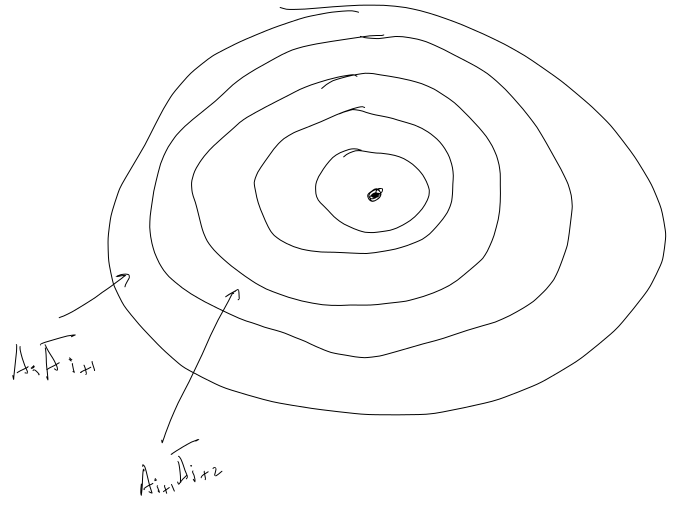
\includegraphics[scale=0.3]{2_1.png}
\end{center}
\[ A_n = \sum_{i = n}^{+ \infty} A_i\overline{A_{i + 1}} \cup \bigcap_{i = n}^{+ \infty}A_i \]
т.к. эти события несовместны
\[ P(A_n) = \sum_{i = n}^{+ \infty}P(A_i\overline{A_{i + 1}}) + P(\bigcap_{i = n}^{+\infty} A_i) \]
т.к. \(P(\bigcap_{i = 1}^{ + \infty} A_i) = \emptyset\) и \(\bigcap_{i = n}^{ +\infty}A_i = \bigcap_{i = 1}^{ + \infty}A_i\), то \(P(\bigcap_{i = n}^{ + \infty} A_i) = 0\) \\
\[ P(A_n) = \sum_{i = n}^{ + \infty} P(A_i \overline{A_{i + 1}}) \]
\[ \sum_{i = 1}^{ + \infty}P(A_i\overline{A_{i + 1}}) = P(A_i) \]
\[ P(A_n) \xrightarrow[n \to + \infty]{} 0 \]
\end{proof}
\begin{remark}
Аксимома счетной аддитивности следует из аксиомы непрерывности и свойства конечной аддитивности
\end{remark}
\subsection{Свойства операция сложения, умножения}
\label{sec:orgab478f1}
\begin{definition}
\-
\begin{enumerate}
\item Свойство дистрибутивности \(A\cdot (B + C) = AB + AC\)
\item Формула сложения. Если \(A\) и \(B\) --- несовместны, то \(P(A + B) = P(A) + P(B)\) \\
если совместны, то \(P(A + B) = P(A) + P(B) - P(AB)\)
\begin{proof}
\-
\begin{center}
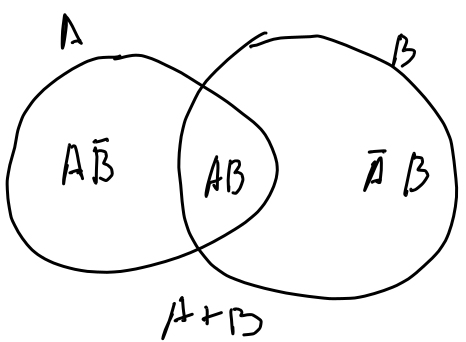
\includegraphics[scale=0.4]{2_2.png}
\end{center}
\[ A + B = A\overline{B} + AB + \overline{A}B \Rightarrow P(A + B) = P(A\overline{B}) + P(AB) + P(\overline{A}B) = \]
\[ = P(A\overline{B}) + P(AB) + (P(\overline{A}B) + P(AB)) - P(AB) = P(A) + P(B) - P(AB) \]
\end{proof}
\end{enumerate}
\end{definition}
\begin{task}
\(n\) писем раскладываются в \(n\) конвертов. Найти вероятнсоть того что
хотя бы одно письмо попадет в свой коверт. Чему равна эта вероятность
при \(n \to + \infty\)
\end{task}
\begin{solution}
\(A_i\) --- \(i\) письмо попало в свой коверт \\
\(A\) --- хотя бы одно письмо попало в свой конверт
\[ A = A_1 + A_2 + \dots + A_n \]
\[ P(A_i) = \frac{1}{n},\ P(A_iA_j) = \frac{1}{A^2_n},\ P(A_iA_jA_k) = \frac{1}{A^3_n}, \dots P(A_1A_2\dots A_n) = \frac{1}{n!}\]
\[ P(A) = n\cdot\frac{1}{n} - C^2_n\cdot\frac{1}{A^2_n} + \dots + (-1)^{n + 1}\frac{1}{n!} = 1 - \frac{1}{2!} + \frac{1}{3!} - \dots + (-1)^{n + 1}\frac{1}{n!} \]
\[ e^{-1} = 1 - 1 + \frac{1}{2!} - \frac{1}{3!} + \dots \]
\[ P(A) \xrightarrow[n \to +\infty]{} 1 - e^{-1} \]
\end{solution}
\subsection{Независимые события}
\label{sec:orge251bc5}
\begin{remark}
\(\Omega = n\), \(|A| = m_1\), \(|B| = m_2\) \\
\(|\Omega \times \Omega| = n^2\), \(AB = m_1m_2\)
\end{remark}
\begin{definition}
События \(A\) и \(B\) называются \textbf{независимыми}, если \(P(AB) = P(A)P(B)\)
\end{definition}
\begin{remark}
Свойство: если \(A\) и \(B\) --- независимы, то \(A\) и \(\overline{B}\) --- независимы
\end{remark}
\begin{proof}
\(P(A) = P(A(B + \overline{B})) = P(AB + A\overline{B}) = P(AB) + P(A\overline{B}) \Rightarrow P(A\overline{B}) = P(A) - P(AB) = P(A) - P(A)\cdot P(B) = P(A)\cdot(1 - P(B)) = P(A)\cdot P(\overline{B})\) \(\Rightarrow\) \(A\) и \(\overline{B}\) --- независимы
\end{proof}
\begin{definition}
События \(A_1,A_2, \dots, A_n\) называются \textbf{независимыми в совокупности}, если для любого набора \(1 \le i_1, i_2, \dots, i_k \le n\ P(A_{i_1}A_{i_2}\dots A_{i_k}) = P(A_{i_1})P(A_{i_2})\dots P(A_{i_k})\)
\end{definition}
\begin{remark}
Если события независимы в совокупности, то события независимы попарно(при \(k = 2\)). Обратное неверно
\end{remark}
\begin{examp}[Берштейна]
Три грани правильного тетраэдра выкрашены в красный, синий, зленый цвета, а четвертая грань во все эти три цвета \\
\(] A\) --- грань содержит красный цвет, \(B\) --- синий, \(C\) --- зеленый \\
\[ P(A) = P(B) = P(C) = \frac{2}{4} = \frac{1}{2} \]
\[ P(AB) = P(AC) = P(BC) = \frac{1}{4} \]
\[ P(AB) = \frac{1}{4} = \frac{1}{2}\cdot\frac{1}{2} = P(A)P(B) \] \(\Rightarrow\) все события попарно независимы
\[ P(ABC) = \frac{1}{4} \neq P(A)P(B)P(C) = \frac{1}{8} \] \(\Rightarrow\) события не независимы в совокупности
\end{examp}
\begin{remark}
Если в условии есть ``хотябы``, т.е. требуется найти вероятность совместных независимых событий, то применяем формулу обратной вероятности
\end{remark}
\begin{task}
Найти веротяность того, что при 4 бросаниях кости, хотябы один раз выпадет шестерка.
\end{task}
\begin{solution}
\(] A_1\) --- при 1 броске ``6``, \(A_2\) --- при 2х бросках ``6``, \dots{}, \(A\) --- хотя бы один раз ``6``
\[ A = A_1 + A_2 + A_3 + A_4 \]
\[ P(A_1) = P(A_2) = P(A_3) = P(A_4) = \frac{1}{6} \]
\[ P(\overline{A_1}) = P(\overline{A_2}) = P(\overline{A_3}) = P(\overline{A_4}) = \frac{5}{6} \]
\(\overline{A}\) --- ни разу не выпадет
\[ \overline{A} = \overline{A_1}\cdot\overline{A_2}\cdot\overline{A_3}\cdot\overline{A_4} \]
\[ P(\overline{A}) = \left(\frac{5}{6}\right)^4  \]
\[ P(A) = 1 - P(\overline{A}) \]
\end{solution}
\begin{task}
Два стрелка стреляют по мишени. Вероятность попадания первого --- \(0.6\), второго --- \(0.8\)
\end{task}
\begin{solution}
\(A_1\) --- 1й попал \\
\(A_2\) --- 2й попал \\
\(A\) --- один попал
\[ A = A_1\cdot\overline{A_2} + \overline{A_1}\cdot A_2 \]
\[ P(A)  = P(A)\cdot P(\overline{A_2}) + P(\overline{A_1})\cdot P(A_2) \]
\end{solution}
\chapter{}
\label{sec:orgba63f8a}
\section{Условная вероятность}
\label{sec:org53656e8}
\begin{symb}
\(P(A | B)\) --- вероятность наступления события \(A\), вычисленная в предположении, что событие \(B\) уже произошло
\end{symb}
\begin{examp}
Кубик подбрасывается один раз. Известно что выпало больше трех очков. Найти вероятность того, что выпало четное число очков.
\begin{itemize}
\item \(A\) --- четное число очков
\item \(B\) --- больше 3 очков
\end{itemize}
Тогда:
\begin{itemize}
\item \(n = 3\) \((4, 5, 6)\)
\item \(m = 2\) \((4, 6)\)
\end{itemize}
\[ P(A|B) = \frac{2}{3} = \frac{\frac{2}{6}}{\frac{3}{6}} = \frac{P(A\cdot B)}{P(B)}\]
\end{examp}
\noindentПри интерпретация с геометрическим определением вероятностей также получаем формулу \(P(A|B) = \frac{P(A\cdot B)}{P(B)}\)
\begin{definition}
\textbf{Условной вероятностью} события \(A\) при условии того что имело место событие \(B\) называется величина:
\[ P(A|B) = \frac{P(A \cdot B)}{P(B)} \] --- \textbf{формула условной вероятности}
\end{definition}
\subsection{Формула умножения вероятности}
\label{sec:org4a59c9e}
Как следствие формулы условной вероятности получаем:
\[ P(AB) = P(B) \cdot P(A|B)  \text{ или } P(AB) = P(A)\cdot P(B | A)\]
\begin{theorem}
\[ P(A_1 A_2 \dots A_n) = P(A_1) \cdot P(A_2 | A_1) \cdot P(A_3 | A_1 A_2) \dots P(A_n | A_1\dots A_{n - 1})\]
\end{theorem}
\begin{proof}
По индукции
\end{proof}
\begin{remark}
\(P(A) \neq 0\) и поэтому формула умножения удовлетворяет
\[ P(A_1 A_2 \dots A_n) \neq 0\]
\end{remark}
\begin{remark}
\[ P(A|B) = P(A) \Leftrightarrow P(AB) = P(A) \cdot P(B) \]
\end{remark}
\begin{proof}
Очевидно
\end{proof}
\begin{task}
В коробке 3 красных крандаша и 2 синих. Вынули 3 карандаша. Найти вероятность того что первые два красные а третий синий.
\end{task}
\begin{solution}
\-
\begin{itemize}
\item \(A_1\) --- 1-й красный
\item \(A_2\) --- 2-й красный
\item \(A_3\) --- 3-й синий
\end{itemize}
\[ P(A_1 A_2 A_3) = P(A_1) \cdot P(A_2 | A_1) \cdot P(A_3 | A_2 A_1) = \frac{3}{5} \cdot \frac{2}{4} \cdot \frac{2}{3} = \frac{1}{5} = 0.2\]
\end{solution}
\begin{remark}
Прменяем когда учитывается порядок
\end{remark}
\subsection{Полная группа событий}
\label{sec:org5fb0edd}
\begin{definition}
События \(H_1, H_2, \dots, H_n, \dots\) образуюти полную группу событий если они попарно несовместны, и содержат все элементарные исходы:
\begin{itemize}
\item \(P(H_i H_j) = \emptyset\ \forall i \neq j\)
\item \(\sum\limits_{i = 1}^\infty H_i = \Omega\)
\end{itemize}
\end{definition}
\begin{remark}
Часто события из полной группы называются гипотезами
\end{remark}
\subsection{Формула полной вероятности}
\label{sec:org8e02495}
\begin{theorem}[Баеса]
\(] H_1, H_2, \dots, H_n ,\dots\) --- полная группа событий \\
\uline{Тогда} \[ P(H_k|A) = \frac{P(H_k)P(A|H_k)}{\sum_{i = 1}^{\infty}P(H_i)P(A|H_i)} \]
\end{theorem}
\begin{examp}
В первой коробке 4 белых и два черных шара, во второй 1 белый и два
черных. Из первой коробки во вторую переложили два шара, затем из
второй коробки достали шар. Найти вероятность того что он оказался белый
\end{examp}
\begin{solution}
\-
\begin{itemize}
\item \(] H_1\) --- переложили 2 белых
\item \(] H_2\) --- переложили 2 черных
\item \(] H_3\) --- переложили 1 черный и 1 белый
\item \(] A\) --- из второй коробки достали белый
\end{itemize}
\[ P(H_1) = \frac{4}{6}\cdot\frac{3}{5} =  \frac{6}{15} \]
\[ P(H_2) = \frac{2}{6}\cdot\frac{1}{5} = \frac{1}{15} \]
\[ P(H_3) = \frac{4}{6}\cdot\frac{2}{5} + \frac{2}{6}\cdot\frac{4}{5} = \frac{8}{15} \]
\[ \sum P(H_i) = 1\text{ --- верно} \]
\[ P(A|H_1) = \frac{3}{5} \]
\[ P(A|H_2) = \frac{1}{5} \]
\[ P(A|H_3) = \frac{2}{5} \]
По формуле полной вероятности:
\[ P(A) = P(H_1)\cdotP(A|H_1) + P(H_2)\cdotP(A|H_2) + P(H_3)\cdotP(A|H_3) = \frac{6}{15}\cdot\frac{3}{5} + \frac{1}{15}\cdot\frac{1}{5} + \frac{8}{15}\cdot\frac{2}{5} = \frac{7}{15}\]
\end{solution}
\begin{task}
По статистике 1\% населения болен раком. Тест дает правильный результат
в 99\% случаев. Тест оказался положительным. Найти веротяность того что
человек болен.
\end{task}
\begin{solution}
$]$ \left.\begin{array}{l}
$H_1$ --- болен \\
$H_2$ --- здоров
\end{array}\right\}
, \(A\) --- тест положительный
\begin{itemize}
\item \(P(H_1) = 0.01\)
\item \(P(H_2) = 0.99\)
\item \(P(A|H_1) = 0.99\)
\item \(P(A|H_2) = 0.01\)
\[ P(H_1|A) = \frac{P(H_1)P(A|H_1)}{P(H_1)P(A|H_1) + P(H_2)P(A|H_2)} = \frac{1}{2} \]
\end{itemize}
Сделаем второй тест:
\begin{itemize}
\item \(P(H_1) = 0.01\)
\item \(P(H_2) = 0.99\)
\item \(P(AA|H_1) = 0.99^2\)
\item \(P(AA|H_2) = 0.01^2\)
\end{itemize}
\[ P(H_1|AA) = \frac{0.99}{0.99 + 0.01} = 0.99 \]
\end{solution}
\chapter{}
\label{sec:org5e22154}
\section{Схема Бернулли}
\label{sec:org4f52906}
\begin{definition}
Схемой Бернулли называется серия независимых испытаний, каждое из
которых имеет два исхода, каждое интересующее нас событие лиибо
произошло либо не произошло.
\begin{itemize}
\item \(n\) --- число испытаний
\item \(p\) --- вероятность события \(A\) при одном испытании
\item \(q = 1 - p\)
\item \(\nu_k\) --- число успехов при \(k\) испытаниях
\item \(P_n(k) = P(\nu_k = k)\)
\end{itemize}
\end{definition}
\begin{theorem}
Вероятность того что при \(n\) испытаниях произойдет ровно \(k\) успехов равна:
\[ P_n(k) = C^k_np^kq^{n - k} \]
\end{theorem}
\begin{proof}
Рассмотрим один из исходов благоприятных событию \(A\): \(A_1 = \underbrace{\text{УУ}\dots\text{У}}_k\underbrace{\text{НН}\dots\text{Н}}_{n - k}\) --- независмые события \\
\begin{itemize}
\item \(P(\text{У}) = p\)
\item \(P(\text{Н}) = q\)
\end{itemize}
\[ P(A_1) = \underbrace{pp\dots p}_k\underbrace{qq\dots q}_{n - k} = p^kq^{n - k} \]
\[ P(A) = C^k_np^kq^{n - k} \]
\end{proof}
\begin{task}
Вероятность попадания стрелка в цель при одном выстреле 0.8. Найти
вероятность того что при 5 выстрелах будут 3 попадания
\end{task}
\begin{solution}
\-
\begin{itemize}
\item \(n = 5\)
\item \(p = 0.8\)
\item \(q = 0.2\)
\item \(k = 3\)
\end{itemize}
\[ P_5(3) = C^3_5 p^3q^2 = 0.2048\]
\end{solution}
\subsection{Наиболее вероятное число успехов}
\label{sec:org7a51972}
Выясним при каком значении \(k\) вероятность предшествующего числа
успехов \(k - 1\) будет не больше чем веротяность \(k\) успехов
\[ P_n(k - 1) \le P_n(k) \]
\[ C^{k-1}_np^{k - 1}q^{n - k + 1} \le C^k_np^kq{n - k} \]
\[ \frac{n!}{(k - 1)!(n -k + 1)!}q \le \frac{n!}{(k!(n - k)!)}p \]
\[ \frac{k!}{(k-1)!}q \le \frac{(n - k + 1)!}{(n - k)!}p \]
\[ k(1- p) \le (n - k + 1)p \]
\[ k \le np + p \]
Так как \(k\) --- целое то выполняется: \(np + p - 1\le k \le np + p\) \\
Рассмотрим три ситуации:
\begin{enumerate}
\item \(np\) --- целое. Тогда \(np + p\) --- целое и \(k = np\) --- наиболее вероятное число исходов
\item \(np + p\) --- не целое. Тогда \(k = [np + p]\)
\item \(np + p\) --- целое. Тогд \(np + p - 1\) --- целое и \(P_n(k - 1)
   = P_n(k)\) и имеем два наиболее вероятных числа успехов:
\begin{itemize}
\item \(k = np + p\)
\item \(k = np + p - 1\)
\end{itemize}
\end{enumerate}
\begin{center}
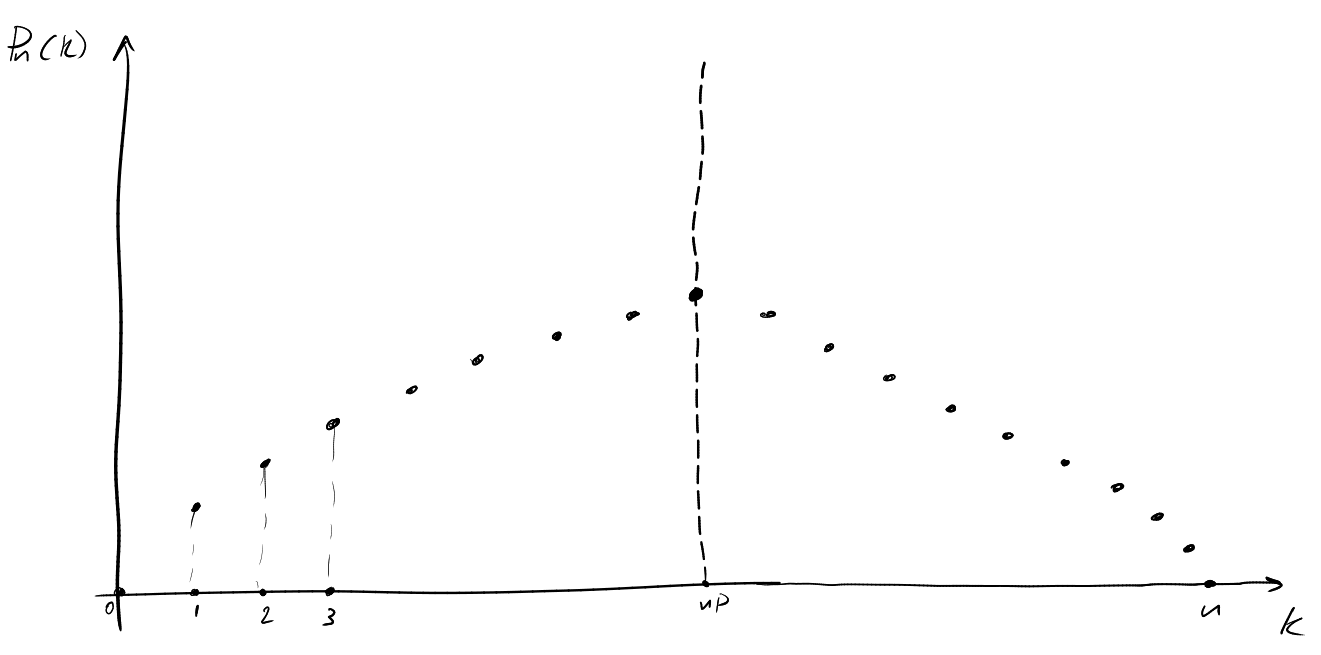
\includegraphics[scale=0.35]{4_1.png}
\end{center}
\subsection{Предельные теоремы в схеме Бернулли}
\label{sec:org333f380}
\begin{definition}
\textbf{Локальная формула} Муавра-Лапласса. Применяем когда требуется найти вероятноть точного числа успехов.
\[ P_n(\nu_n = k) \approx \frac{1}{\sqrt{npq}}\varphi(x) \]
, где \(\varphi(x) = \frac{1}{\sqrt{2\pi}}e^{-\frac{x^2}{2}}, x = \frac{k - np}{\sqrt{npq}}\) --- функция Гауса. \\
Свойства функции Гауса \(\varphi(x)\):
\begin{enumerate}
\item \(\varphi(-x) = \varphi(x)\) --- четная
\item при \(x > 5,\ \varphi(x) \approx 0\)
\end{enumerate}
\end{definition}
\begin{definition}
\textbf{Интегральная формула Лапласса}. Применяем если число успехов лежит в неком диапозоне.
\[ P_n(k_1 \le \nu_n \le k_2) \approx \Phi(x_1) - \Phi(x_2) \]
, где \[ \Phi(x) = \frac{1}{\sqrt{2\pi}} \int_0^x e^{-\frac{z^2}{2}} dz\] --- функция Лапласса \\
\[ x_1 = \frac{k_1 - np}{\sqrt{npq}},\ x_2 = \frac{k_2 - np}{\sqrt{npq}} \]

Свойства \(\Phi(x)\):
\begin{enumerate}
\item \(\Phi(-x) = \Phi(x)\) --- нечетная
\item при \(x > 5,\ \Phi(x) \approx 0.5\)
\end{enumerate}
\end{definition}
\begin{remark}
В некоторых источниках под функцией Лапласса подразумевается несколько иная функция, чаще всего:
\[ F_0(x) = \frac{1}{\sqrt{2\pi}} \int_{-\infty}^x e^{z^2}{2}dz \]
\[ F_0(x) = 0.5 + \Phi(x)\text{ или }\Phi(x) = F_0(x)-0.5 \]
\end{remark}
\begin{remark}
Формулу применяем при \(n \ge 100\) и \(p,q\ge0.1\) 
\end{remark}
\begin{task}
Вероятность попадания стрелка в цель при одном выстреле 0.8. Стрелок сделал 400 выстрелов. Найти вероятность того что
\begin{enumerate}
\item произошло ровно 330 попаданий
\item произошло от 312 до 336 попаданий
\end{enumerate}
\end{task}
\begin{solution}
\-
\begin{enumerate}
\item \(n = 400, p = 0.8, q = 0.2, k=330\)
\[ x = \frac{330 - 400\cdot0.8}{\sqrt{400\cdot0.8\cdot0.2}} = 1.25 \]
\[ P_{400}(330) \approx \frac{1}{8} \cdot \varphi(1.25) \approx \frac{1}{8}\cdot0.1826 \approx 0.0228 \]
\item \(n = 400, p=0.8, q = 0.2, k_1 =312, k_2 = 336\)
\[ x_1 = \frac{312 - 400\cdot0.8}{\sqrt{400\cdot0.8\cdot0.2}} = -1\]
\[ x_2 = \frac{336 - 400\cdot0.8}{\sqrt{400\cdot0.8\cdot0.2}} = 2\]
\[ P_{400}(312 \le \nu_n \le 336) = \Phi(2) - \Phi(-1) = \Phi(2) + \Phi(1) \approx 0.8185 \]
\end{enumerate}
\end{solution}
\section{Статистическое определение вероятности}
\label{sec:orgbf1412b}
\begin{itemize}
\item \(n_A\) --- число появления события \(A\) при \(n\) испытаниях
\item \(\frac{n_A}{n}\) --- частота события \(A\)
\end{itemize}
\[ P(A) \approx \frac{n_A}{n}, \text{при }n\to\infty \]

\subsection{Вероятность отклонения относительной частоты}
\label{sec:orgceaf4c2}
\(] p\) --- веротяность события \(A\), \(\frac{n_A}{n}\) --- частота \(A\) \\
По интегральной формуле Лапласса:
\[ P\left(\left|\frac{n_A}{n} - p| \le \varepsilon\right) = P(-\varepsilon \le \frac{n_A}{n} - p \le \varepsilon) = P(-n\varepsilon \le n_a - np \le n\varepsilon) = P(np - n\varepsilon \le n_A \le np + n\varpepsilon) \]
\[ x_1 = \frac{np - n\varepsilon - np}{\sqrt{npq}} = -\frac{n\varepsilon}{\sqrt{npq}} \]
\[ x_2 = \frac{np + n\varepsilon - np}{\sqrt{npq}} = \frac{n\varespilon}{\sqrt{npq}} \]
\[ P\left(\left|\frac{n_A}{n} - p\right| \le \varepsilon\right) = \Phi\left(\frac{n\varepsilon}{\sqrt{npq}}\right) - \Phi\left(-\frac{n\varepsilon}{\sqrt{npq}}\right) = 2\Phi\left(\frac{n\varepsilon}{\sqrt{npq}}\right) \]
\[ P\left(\left|\frac{n_A}{n} - p\right| \le \varepsilon\right) = 2\Phi\left(\frac{\sqrt{n}}{\sqrt{pq}}\varepsilon\right) \]
\subsection{Закон больших чисел Бернулли}
\label{sec:org6ab1a82}
Более точно последняя формула выглядит так:
\[ P\left(\left|\frac{n_A}{n} - p\right| \le \varepsilon\right) \xrightarrow[n \to \infty]{} 2\Phi\left(\frac{\sqrt{n}}{\sqrt{pq}}\varepsilon\right) \]
при \(n \to \infty\) \(\frac{\sqrt{n}}{\sqrt{pq}}\varepsilon \to \infty\) и \(\Phi\left(\frac{\sqrt{n}}{\sqrt{pq}}\right) \to 0.5\)
\[ P\left(\left|\frac{n_A}{n} - p\right| \le \varepsilon\right) \to 2\cdot0.5 = 1\]
\[ \lim_{n\to\infty}P\left(\left|\frac{n_A}{n} - p \right| \le \varepsilon \right) = 1 \]
--- закон больших чисел Бернулли \\
То есть при большом числе испытаний, будет близко к реальной вероятности
\chapter{}
\label{sec:orgbf3f443}
\section{Схемы испытаний и соответствующие распределения}
\label{sec:orgdf587ad}
\begin{itemize}
\item \(n\) --- число испытаний
\item \(p\) --- вероятность при одном испытании
\item \(q = 1 - p\) --- вероятность неудачи при одном испытании
\end{itemize}


\begin{definition}
\[ k \to C^k_n p^k q^{n - k} \] --- биноминальное распределение с параметрами \(n\) и \(p\)
\end{definition}
\begin{symb}
\(B_{n,p} = B(n, p)\)
\end{symb}
\subsection{Схема до первого успешного испытания}
\label{sec:org69399d3}
\begin{definition}
\textbf{Схема до первого успешного испытания}. Пусть проводится бесконечная
 серия испытаний, которая заканчивается после первого успеха под номером \(\tau\)
\end{definition}
\begin{theorem}
\(p(\tau = k) = q^{k - 1}p\)
\end{theorem}
\begin{proof}
\[ p(\tau = k) = p(\underbrace{\text{НН}\dots\text{Н}}_{k - 1}\underset{\substack{\uparrow \\ k}}{\text{У}}) = q^{k - 1}p\]
\end{proof}
\begin{definition}
\(k \to q^{k-1}p,\ 1 \le k \le \infty\) --- называется \textbf{геометрическим распределением} с параметром \(t\)
\end{definition}
\begin{symb}
G(p)
\end{symb}
\begin{remark}
Это распределение обладает так назыаемым свойством отсутствия после действия или свойством нестарения
\end{remark}
\begin{theorem}
\(] p(\tau = k) = q^{k - 1}p\) \\
\uline{Тогда} \(\forall n, k \in \N\ p(\tau > n + k| \tau > n) = p(\tau > k)\)
\end{theorem}
\begin{proof}
По формуле условной вероятности: \[ p(\tau > n + k |\tau > k) = \frac{p(\tau > n + k \text{ и } \tau > j)}{p(\tau > n)} = \frac{p(\tau > n + k)}{p(\tau > n)} \addtag\label{5_1_geom} \]
\(p(\tau > m) = p(\text{первые } m\text{ неудач}) = q^m\)
\[ \ref{5_1_geom} = \frac{q^{n + k}}{q^n} = q^k \]
\end{proof}
\begin{remark}
То, проработет ли девайс \(k\) часов после этого, не зависит от того сколько проработал до этого
\end{remark}
\begin{remark}
Также \(p(\tau = n + k|\tau > n) = p(\tau = k)\)
\end{remark}
\subsection{Испытание с несколькими исходами}
\label{sec:org8b789cb}
Пусть при \(n\) испытаниях могут произойти \(m\) несовместных исходов
\begin{itemize}
\item \(p_i\) --- вероятность \(i\)-го исхода при одном отдельном испытании
\end{itemize}
\begin{theorem}
Вероятность того, что при \(n\) испытаниях первый исход появится \(n_1\) раз, второй \(n_2\) раз, \dots{}, \(m\)-й \(n_m\) раз. \(n_1 + n_2 + \dots + n_m = n\)
\uline{Тогда} \[ p(n_1, n_2, \dots, n_m) = \frac{n!}{n_1!n_2!\dots n_m!}p_1^{n_1}p_2^{n_2}\dots p_m^{n_m} \]
\end{theorem}
\begin{proof}
\(A_1 = \underbrace{11\dots1}_{n_1}\underbrace{22\dots2}_{n_2}\dots \underbrace{m\dots m}_{n_m}\)
\[ p(A_1) = p_1^{n_1}\dots p_n^{n_m} \]
Остальные благоприятные исходы отличаются лишь расположением \(i\)-х исходов по \(n\) местам, а веротяности будут те-же. Всего таких исходов будет:
\[ C^{n_1}_nC^{n_2}_{n - n_1}C^{n_3}_{n - n_1 - n_2}\dots C^{n_m}_{n_m} = \frac{n!}{n_1!n_2!\dots n_m!} \] --- формула для перестановок с повторениями
\end{proof}
\begin{task}
Два одинаковых по силе шахматиста играют матч из 6 партий. Вероятность ничьи при одной партии --- \(0.5\). Найти веротяность того, что второй игрок две партии выиграл, а три партии свел в ничью
\end{task}
\begin{solution}
Исходы:
\begin{enumerate}
\item первый выиграл
\item второй выиграл
\item ничья
\[ p_3 = \frac{1}{2};\ p_1 = p_2 = \frac{1}{2}\left(1 - \frac{1}{2}\right) = \frac{1}{4};\ n= 6 \]
\[ P(1, 2, 3) = \frac{6!}{1!2!3!}\cdot\left(\frac{1}{4}\right)^1\cdot\left(\frac{1}{4}\right)^2\cdot\left(\frac{1}{2}\right)^3  = \frac{15}{2^7}\]
\end{enumerate}
\end{solution}
\subsection{Урновая схема}
\label{sec:orgf1fc38d}
В урне \(N\) шаров. Из них \(K\) белых, а черных \(N - K\). Из нее выбираем \(n\) шаров без учета порядка. \(k\) --- число вынутых белых
\begin{theorem}[Схема с возвратом]
Вероятность вынуть белый шар не менятеся. \\
\uline{Тогда} \[ p = \frac{K}{N}\quad p_n(k) = C^k_np^k(1 - p)^{n - k} \]
--- биноминальное распределение
\end{theorem}
\begin{theorem}[Схема без возврата]
\uline{Тогда} \[ P_{N,K}(n, k) = \frac{C^k_K\cdot C^{n-k}_{N - K}}{C^n_N} \]
\end{theorem}
\begin{definition}
\[ k \to \frac{C^k_K\cdot C^{n - k}_{N - K}}{C^n_N},\ k \le K \]
назвается \textbf{гипергеометрическим} распределением веротяности
\end{definition}
\begin{lemma}
\[ C^k_K \sim \frac{K^k}{k!} \]
, при \(K \to \infty, K = \const\)
\end{lemma}
\begin{proof}
\[ C^k_K = \frac{K!}{k!(K - k)!} = \frac{K(K - 1)\dots(K - k + 1)}{K^k}\cdot \frac{K^k}{k!} = \]
\[ = \underbrace{1 \cdot \left(1 - \frac{1}{K}\right)\cdot\left(1 - \frac{2}{K}\right) \dots \left(1 - \frac{k - 1}{K}\right)}_{\substack{\downarrow \\ 1}} \cdot\frac{K^k}{k!} \sim \frac{K^k}{k!}\]
\end{proof}
\begin{theorem}
\-
\begin{itemize}
\item \(N \to \infty\)
\item \(K \to \infty\)
\item \(\frac{K}{N} \to p \in (0, 1)\)
\item \(n\) и \(0 \le k \le K\) --- фиксированны
\end{itemize}
\uline{Тогда} \[ P_{N,K}(n,k) = \frac{C^k_KC^{n - k}_{N - K}}{C^n_N} \to C^k_np^k(1 - p)^{n - k} \]
\end{theorem}
\begin{proof}
\[ P_{N, K}(n, k) = \frac{C^k_KC^{n - k}_{N - K}}{C^n_N} \xrightarrow[N \to \infty]{} \frac{K^k}{k!}\cdot \frac{(N -K)^{n - k}}{(n - k)!}\cdot \frac{n!}{N^n} = \frac{n!}{k!\cdot(n- k)!}\cdot \frac{K^k}{N^k}\cdot\frac{(N - K)^{n - k}}{N^{n - k}} = \]
\[ = C^k_n\left(\frac{K}{N}\right)^k\left(1 - \frac{K}{N}\right)^{n -k} \xrightarrow[N \to \infty]{} C^k_n\cdot p^k \cdot ( 1- p)^{n - k}\]
\end{proof}
\subsection{Схемы Пуассона. Теорема Пуассона для схемы Бернулли}
\label{sec:orgde39229}
Схема: вероятность успеха при одном отдельном испытании зависит от числа испытаний \(n\) таким образом, чтобы \(n \cdot p_n = \lambda\)(точнее \(np_n \xrightarrow[n \to \infty]{} \lambda\)) \\
Появление очень редких событий в длинном потоке испытаний
\begin{theorem}[Формула Пуассона]
Пусть \(n \to \infty,\ p_n \to 0\), так что \(np_n \to \lambda > 0\) \\
\uline{Тогда} вероятность \(k\) успехов при \(n\) испытаниях \[p(\nu_n = k) = C^k_np_n^k(1 - p_n)^{n -k} \xrightarrow[n \to \infty]{} \frac{\lambda^k}{k!}e^{-\lambda}\]
\end{theorem}
\begin{proof}
Положим \(\lambda_n = np_n\)
\[ p(\nu_n = k) = C^k_np_n^k(1 - p_n)^{n - k} \xrightarrow[n \to \infty]{} \frac{n^k}{k!}\cdot \frac{\lambda_n^k}{n^k}\cdot\left(1 - \frac{\lambda_n}{n}\right)^{n - k} = \frac{\lambda_n^k}{k!}\cdot\left(1 - \frac{\lambda_n}{n}\right)^n\cdot\left(1 - \frac{\lambda_n}{n}\right)^{-k} \xrightarrow[n \to \infty]{} \]
\[ \xrightarrow[n \to \infty]{} \frac{\lambda_n^k}{k!}\cdot\left(1 - \frac{\lambda_n}{n}\right)^n \xrightarrow[n \to \infty]{} \frac{\lambda_n^k}{k!}\cdot\left(\left(1 - \frac{\lambda_n}{n}\right)^{-\frac{n}{\lambda_n}}\right)^{-\lambda_n} \xrightarrow[n \to \infty]{} \frac{\lambda_n^k}{k!}e^{-\lambda_n} \xrightarrow[n \to \infty]{} \frac{\lambda^k}{k!}e^{-\lambda} \]
\end{proof}
\begin{enumerate}
\item Оценка погрешности в формуле Пуссона
\label{sec:orgebdd362}
\begin{theorem}
Пусть \(\nu_n\) -- число успехов при \(n\) испытаниях в схеме Бернулли с вероятностью \(p\)
\[ \lambda = np\quad A \subset \{0, 1, 2, \dotsm n\}\text{ --- произвольное подмножество}\]
\uline{Тогда} погрешность
\[ \left|p(\nu_n \in A) - \sum_{k \in A} \frac{\lambda_k}{k!} e^{-\lambda}\right| \le \min(p, \lambda p) = \min(p, np^2) = \min\left(p, \frac{\lambda^2}{n}\right) \]
\end{theorem}
\begin{remark}
Формулу Пуасснона иногда называют формулой редких событий. Применяем при малых \(p\), \(n \ge 100\)
\end{remark}
\begin{task}
Прибор состоит из 1000 элементов. Вероятность отказа каждого элемента \(\frac{1}{1000}\). Какова вероятность отказа больше двух элементов
\end{task}
\begin{solution}
\[ p_n(k) \approx \frac{\lambda^k}{k!}e^{-\lambda} \]
, где \(\lambda = np\)
\begin{itemize}
\item \(n = 1000\)
\item \(p = 0.001\)
\item \(\lambda = np = 1\)
\item \(k > 2\)
\end{itemize}
\[ p(\nu_n > 2) = 1 - p(\nu_n \le 2) = 1 - (p(0) + p(1) + p(2)) \approx 1 - \left(\frac{\lambda^0}{0!} e^{-\lambda} + \frac{\lambda^1}{1!}e^{-\lambda} + \frac{\lambda^2}{2!}e^{-\lambda}\right) = \]
\[ = 1 - 2.5e^{-1} \approx 0.0803\]
Погрешность \(\varepsilon \le \min(p, \lambda p) = 0.001\)
\end{solution}
\end{enumerate}
\chapter{}
\label{sec:orga74d6c2}
\newcommand{\todo}{{\color{red}\text{Доделать }}}
\newcommand{\fixme}{{\color{red}\text{Исправить }}}


\section{Случайные величины}
\label{sec:org1ebd8ff}
\begin{symb}
\(\xi\) --- \textbf{Случаная величина}
\end{symb}
\begin{examp}
\(\xi\) --- число выпавших очков. \(\xi \in \{1, 2, 3, 4, 5, 6\}\)
\end{examp}
\begin{examp}
\(\xi\) --- время работы микросхемы до отказа
\begin{enumerate}
\item Время работы в часах \\
\(\xi = \{1, 2, 3, \dots \}\)
\item Время работы измеряем точно \\
\(\xi \in [0, +\infty]\)
\end{enumerate}
\end{examp}
\begin{examp}
\(\xi\) --- температура воздуха в случайный момент вермени. \(\xi \in (-50^\circ, 50^\circ)\)
\end{examp}
\begin{examp}
Индикатор события \(A\).
\[I_A(\omega) \in \begin{cases} 0 & , \omega \not \in A \\ 1 & , \omega \in A\end{cases}\]
\end{examp}
\begin{definition}
Пусть имеется вероятностное пространство \((\Omega, \mathcal{F}, p)\). Функция \(\xi: \Omega \to \R\) называется \textbf{\(\mathcal{F}\)-измеримой}, если \(\forall x \in \R:\ \{\omega | \xi(\omega) < x\} \in \mathcal{F}\). Т.е прообраз \(\xi^{-1}((- \infty, x)) \in \mathcal{F}\)
\end{definition}
\begin{definition}
\textbf{Случаной величиной} \(\xi\) заданной на вероятностном пространстве \((\Omega, \mathcal{F}, p)\)  назывется \(\mathcal{F}\)-измеримая функция \fixme, ставящая в соответсвие каждому элементарному исходу \(\omega\) некоторое вещественное число
\end{definition}
\begin{examp}
Бросаем кость.
\begin{itemize}
\item \(\Omega = \{1, 2, 3, 4, 5, 6\}\)
\item \(\mathcal{F} = \{\emptyset, \Omega, \{1, 3, 5\}, \{2, 4, 6\}\}\)
\item \(] \xi(i) = i\)
\end{itemize}
Если \(x = 4\), то \(\{\omega | \xi(\omega) < 4\} = \{1, 2, 3\} \not\in \mathcal{F}\) \(\Rightarrow\) \(\xi\) не является \(\mathcal{F}\)-измеримой
\end{examp}
\subsection{Смысл измеримости}
\label{sec:org407cf25}
Пусть случайная величина \(\xi: \Omega \to \R\) --- измеримая. Тогда \(P(\xi < x) = P(\{\omega | \xi(\omega) < x\})\), т.к. \(A_x = \{\omega | \xi(\omega) < x\} \in \mathcal{F}\). Тогда \[\overline{A_x} = \{\omega | \xi(\omega) \ge x\} \in \mathcal{F}\] \[A_x \setminus B_y = \{\omega | t \le \xi(\omega) le x\} \in \mathcal{F}\]
\[ B_x = \todo \]
\[ B_x \setminus A_x = \{\omega | \xi(\omega) = x\} \in \mathcal{F} \]
Отсюда видим, по теореме Каво?\fixme  можно однозначно продолжить до любого Борелевского множества на прямой. \(B \in \mathcal{B}\) --- Борелевская \(\sigma\)-алгебра. \(P(B \in \mathcal{B}) = P\{\omega | \xi(\omega) \in B\}\) \\
Пусть случаная величина задана на вероятностном пространстве \((\Omega, \mathcal{F}, p)\). Тогда:
\begin{enumerate}
\item \((\Omega, \mathcal{F}, p) \xrightarrow[]{\xi} (\R, \mathcal{B}, p)\) --- новое веротяностное пространство
\item \(\xi^{-1}(B)\ \forall B \in \mathcal{B}\) \\
\(\mathcal{F}_\xi \subset \mathcal{F}\) \\
\(\mathcal{F}_\xi\) --- \(\sigma\)-алгебра порожденная величной \(\xi\)
\end{enumerate}
\begin{task}
Найти \(\sigma\)-алгебру порожденную индикатором
\end{task}
\begin{definition}
Функция \(P(B)\ B \in \mathcal{B}\) называется \textbf{распределнием вероятностей} случаной величниы \(\xi(\omega)\). Т.е. распределение случайной величны это соответсвие множествами на вещественной прямой и вероятностями случаной величны попасть в это множество
\end{definition}
\subsection{Типы распределения}
\label{sec:org3d3f713}
\begin{itemize}
\item Дискретные
\item Абсолютно непрерывные
\item Смешанные
\item Сингулярные (непрерывные но не абсолютно непрерывные)
\end{itemize}
\begin{enumerate}
\item Дискретные
\label{sec:org84eccc1}
Случайная величина \(\xi\) имеет дискретное распределение, если она принимает не более чем счетное число значений, т.е. существует конечный или счетный набор чисел \(\{x_1, x_2, \dots, x_n, \dots\}\), такой что
\begin{enumerate}
\item \(p_i = p(\xi = x_i) > 0\)
\item \(\sum\limits_i p_i = 1\)
\end{enumerate}
\begin{center}
\begin{tabular}{l|lllll}
\(\xi\) & \(x_1\) & \(x_2\) & \(\dots\) & \(x_n\) & \(\dots\)\\
\hline
\(p\) & \(p_1\) & \(p_2\) & \(\dots\) & \(p_n\) & \(\dots\)\\
\end{tabular}
\end{center}
\todo
\begin{examp}
Кость
\begin{center}
\begin{tabular}{l|rrrrrr}
\(\xi\) & 1 & 2 & 3 & 4 & 5 & 6\\
\hline
\(p\) & \(\frac{1}{6}\) & \(\frac{1}{6}\) & \(\frac{1}{6}\) & \(\frac{1}{6}\) & \(\frac{1}{6}\) & \(\frac{1}{6}\)\\
\end{tabular}
\end{center}
\todo
\label{org450a219}
\end{examp}
\begin{enumerate}
\item Основные числовые характеристики
\label{sec:org945c885}
\begin{enumerate}
\item Математическое ожидание(среднее значение)
\label{sec:org1b11c1c}
\begin{defintion}
\textbf{Математическим ожиданием} случаной величины \(\xi\) называется число:
\[ E\xi = \sum\limits_i x_i p_i \] при условии что данный ряд сходится абсолютно, иначе говрят что что математическое ожидание не существует
\end{defintion}
\begin{symb}
E\(\xi\)
\end{symb}
\begin{remark}
Смысл: среднее значение, число вокруг которого группируеются значения случаной величины. Физический смысл: центр масс. Статистический смысл: среднее арифметическое наблюдаемых значений при большои значении реальных экспериментов
\end{remark}
\item Дисперсия
\label{sec:orgbc80e80}
\begin{definition}
\textbf{Дисперсией} \(D\xi\) случайной величины \(\xi\) называется среднее квадратов отклонений ее от математического ожидания
\[ D\xi = E(\xi - E\xi)^2 \] или \[D\xi = \sum\limits_i (x_i - E\xi)^2 p_i \]
При условии что данное среднее значение существует(конечно)
\end{definition}
\begin{remark}
Вычислять дисперсию удобнее по формуле \[ D\xi = E\xi^2 - (E\xi)^2  = \sum\limits_i x_i^2p_i - (E\xi)^2\]
\end{remark}
\begin{remark}
Смысл: квадрат среднего разброса(рассейния) случайной величины около ее математического ожидания
\end{remark}
\item Среднее квадратическое отклонение
\label{sec:org748acf6}
\begin{definition}
\textbf{Средним квадратическим отклонением} (\(\sigma\)\textsubscript{\(\xi\)} = \(\sigma\)(\(\xi\))) случайной величины \(\xi\) называется число
\[ \sigma = \sqrt{D\xi} \]
\end{definition}
\begin{remark}
Смысл: характеризует средний разброс случайной величины около ее математического ожидания
\end{remark}
\begin{examp}
\hyperref[org450a219]{Бросаем кость}
\[ E\xi = 1\cdot \frac{1}{6} + 2 \cdot \frac{1}{6}  + 3 \cdot \frac{1}{6} + 4 \cdot \frac{1}{6} + 5 \cdot \frac{1}{6} + 6 \cdot \frac{1}{6} = 3.5 \]
\[ D\xi = 1^2 \cdot \frac{1}{6} + 2^2 \cdot \frac{1}{6} + 3^2 \cdot \frac{1}{6} + 4^2 \cdot \frac{1}{6} + 5^2 \cdot \frac{1}{6} + 6^2 \cdot \frac{1}{6} - 3.5^2 = 2.92 \]
\[ \sigma = \sqrt{2.92} \approx 1 \neq 1 \]
\end{examp}
\end{enumerate}
\item Свойства математического ожидания и дисперсии
\label{sec:orga3ae1b4}
\begin{definition}
Случайная величина \(\xi\) имеет вырожденное распределение, если \(\xi(\omega) = C = \const\ \forall \omega \in \Omega\) или \(p(\xi = C) = 1\)
\[ E \xi = C = \const \]
\[ D \xi = 0 \]
\end{definition}
\begin{proof}
\todo
\end{proof}
\begin{definition}[Свойство сдвига]
\[E(\xi + C) + E\xi + C\]
\[ D(\xi + C) = D \xi \]
\end{definition}
\begin{proof}
\todo
\end{proof}
\begin{definition}
\[ E(C\xi) = CE\xi \]
\[ D(C\xi) = C^2D\xi \]
\end{definition}
\begin{proof}
\todo
\end{proof}
\begin{definition}
\[ E(\xi + \eta) = E\xi + E\eta \]
\end{definition}
\begin{proof}
\-
\begin{itemize}
\item Пусть \(x_i, y_i\) --- соответсвующие значения случайных величин \(xi\) и \(mu\)
\end{itemize}
\[ E(\xi + \eta) = \sum\limits_{i, j} (x_i + y_j) p(\xi = x_i, \eta = y_j) = \sum\limits_i x_i \sum\limits_j p(\xi = x_i, \eta = y_j) + \sum\limits_j y_j \sum p(\xi = x_i, \eta = y_j) \]
\todo
\end{proof}
\begin{definition}
Дискретные случаные величины \textbf{независимы} если \(\forall i, j\ p(\xi = x_i, \eta = y_j) = p(\xi = x_i) \cdot p(\eta = y_j)\)
\label{org4efa3ab}
\end{definition}
\begin{remark}
Если \(xi\) и \(\eta\) независимы, то
\[ E(\xi\eta) = E\xi\cdot E\eta \]
обратное не верно
\end{remark}
\begin{proof}
\[ E(\xi\eta) = \sum\limits_{ij} (x_i y_j)p(\xi = x_i, \eta = y_j) = \sum\limits_i x_i \sum\limits_j y_j(\xi = x_i, \eta = y_j) = \]
\[ = \sum\limits_i x_i \sum\limits_j y_j p(\xi = x_j)p(\eta = y_j) = \sum\limits_i x_i p(\xi = x_i) \cdot \sum\limits_j y_j p(\eta = y_j) = E\xi \cdot E\eta\]
\end{proof}
\begin{proof}
\[ D\xi = E\xi^2 - (E\xi)^2 \]
\[ D\xi = E(\xi - E\xi)^2 = E(\xi - 2\xi E\xi + (E\xi)^2) = E\xi^2 - 2E\xi E\xi + E(E\xi)^2 = \]
\[ E\xi^2 - 2(E\xi)^2 + (E\xi)^2 = E\xi^2 - (E\xi)^2 \]
\end{proof}
\begin{remark}
\[ D(\xi + \eta) = D\xi + D\eta + 2\text{Cov}(\xi, eta) \]
, где \(\text{Cov}(\xi, \eta) = E(\xi\eta) - E\xi\cdot E\eta\) --- \textbf{ковариация}
\end{remark}
\begin{proof}
\[ D(\xi + \eta) = E(\xi + \eta)^2 - (E(\xi + \eta))^2 = E\xi^2 + 2E\xi\eta + E\eta^2 - (E\xi)^2 - 2E\xi\cdot E\eta - (E\eta)^2 = \]
\[ D\xi + D\eta + 2(E(\xi\eta) - E\xi \cdot E\eta) \]
\end{proof}
\begin{remark}
Если случайные величины \(\xi\) и \(\eta\) независимые, то
\[ D(\xi + \eta) = D\xi + \eta \]
\end{remark}
\begin{proof}
По \hyperref[org4efa3ab]{свойству} \(\text{Cov}(\xi, \eta) = 0\)
\end{proof}
\begin{remark}
Среднее квадратическое отклонение --- минимум отклонения случайной величины от точек вещественной прямой, т.е.
\[ D\xi = \min\limits_a (y - a) \fixme \]
\end{remark}
\begin{proof}
\[ E(\xi - a)^2 = E((\xi - E\xi) + (E\xi - a))^2 = E(\xi - E\xi)^2 + \underbrace{2E(\xi - E\xi)\cdot(E\xi - a)}_0 + (E\xi - a)^2 =  \]
\[ = D\xi + (E\xi - a)^2 \le D\xi \]
\end{proof}
\item Другие числовые характеристики
\label{sec:org3f27284}
\begin{remark}
\[ m_k = E\xi^k \] --- момент \(k\)-того порядка \\
В частности \(m_1 = E\xi\)
\end{remark}
\begin{remark}
\[ E|\xi|^k \] --- абсолютный момент \(k\)-того порядка
\end{remark}
\begin{remark}
\[ \mu_k = E(\xi - E\xi)^k \] --- центральный момент \(k\)-того порядка \\
В частности \(\mu_2 = D\xi\)
\end{remark}
\begin{remark}
\[ E|\xi - E\xi|^2 \] --- абсолютный центральный момент \(k\)-того порядка
\end{remark}
\begin{remark}
Центральные моменты можно выразить через относительные моменты
\todo
\end{remark}
\begin{remark}
\textbf{Модой} \(\text{Mo}\) называется такое значение случайной величины, где вероятность события является наибольшей
\[ p(\xi = \text{Mo}) = \max\limits_i p_i \]
\end{remark}
\begin{definition}
\textbf{Медианой} \(\text{Me}\) называется значение случайной величины такое что, \[p(\xi < \text{Me}) = p(\xi > \text{Me}) = \frac{1}{2}\]
\end{definition}
\end{enumerate}
\end{enumerate}
\end{document}
